\documentclass{article}
\usepackage{amsmath}
\usepackage{amsthm}
\usepackage{graphicx}
\DeclareMathOperator{\Bern}{Bern}
\DeclareMathOperator{\Pois}{Pois}
\newtheorem{lemma}{Lemma}
\title{Poisson Distribution}
\author{zhaof17 }
\date{January 2021}

\begin{document}

\maketitle

\section{Introduction}
An important property for Poisson distribution.
Suppose $P_1 \sim \Pois(c)$, $P_2 \sim \Pois(d)$.
And $P_{\lambda}$ is defined as 
\begin{equation}\label{eq:P_lambda}
    P_{\lambda}(x) = \frac{P_1^{1-\lambda}(x) P_2^{\lambda} (x)}
    {\sum_{y \in \mathcal{X}}
    P_1^{1-\lambda}(y)
    P_2^{\lambda} (y)
    }    
\end{equation}

\begin{enumerate}
    \item $P_{\lambda} \sim \Pois(c^{1-\lambda} d^{\lambda})$
    \item $D_{\mathrm{KL}}(P_{\lambda}||P_1) = c^{1-\lambda}d^{\lambda}\log(\frac{d}{c})^{\lambda} + c-c^{1-\lambda}d^{\lambda}$
    \item $D_{\mathrm{KL}}(P_{\lambda}||P_2) = c^{1-\lambda}d^{\lambda}\log(\frac{c}{d})^{1-\lambda} + d-c^{1-\lambda}d^{\lambda}$
\end{enumerate}
The second property is proved using the KL divergence
of two Poisson distributions. See \cite{kl}
\section{Side Information of Abbe}
This section discusses theoretical deduction and experimental results for \cite{abbe}.

Let $c_1 = \frac{a}{2}, c_2=\frac{b}{2}$. $p_0, p_1$ are two
discrete distributions.
The Abbe's conclusion for side information is solving the following
optimization problem:
\begin{equation}\label{eq:lambda}
    \min_{\lambda \in [0,1]} c_1^{1-\lambda}c_2^{\lambda} +
    c_2^{1-\lambda}c_1^{\lambda} + \gamma \log(\sum_{x\in \mathcal{X}}p^{1-\lambda}_0(x) p^{\lambda}_1(x))
\end{equation}
Let $p_{\lambda}$ be defined as
$$
p_{\lambda}(x) = \frac{p_0^{1-\lambda}(x) p_1^{\lambda} (x)}
{\sum_{x \in \mathcal{X}}p_0^{1-\lambda}(x) p_1^{\lambda} (x)}
$$
After solving $\lambda$ from \eqref{eq:lambda}. The theoretical
threshold is given by
\begin{align}
    I_+ &=\lambda (c_1^{1-\lambda}c_2^{\lambda} -
    c_2^{1-\lambda}c_1^{\lambda})\log\frac{c_2}{c_1}+c_1+c_2\notag \\
    &-c_1^{1-\lambda}c_2^{\lambda} -
    c_2^{1-\lambda}c_1^{\lambda}+\gamma D_{\mathrm{KL}}(p_{\lambda}||p_0) \\
    &=(1-\lambda) (c_1^{1-\lambda}c_2^{\lambda} -
    c_2^{1-\lambda}c_1^{\lambda})\log\frac{c_1}{c_2}+c_1+c_2\notag \\
    &-c_1^{1-\lambda}c_2^{\lambda} -
    c_2^{1-\lambda}c_1^{\lambda}+\gamma D_{\mathrm{KL}}(p_{\lambda}||p_1)
    >1
\end{align}
When $\lambda=\frac{1}{2}$ makes $D_{\mathrm{KL}}(p_{\lambda}||p_0)=
D_{\mathrm{KL}}(p_{\lambda}||p_1)$, the threshold of Abbe is the same as
us.

\subsection{Experiment Result}
\begin{figure}
    \centering
    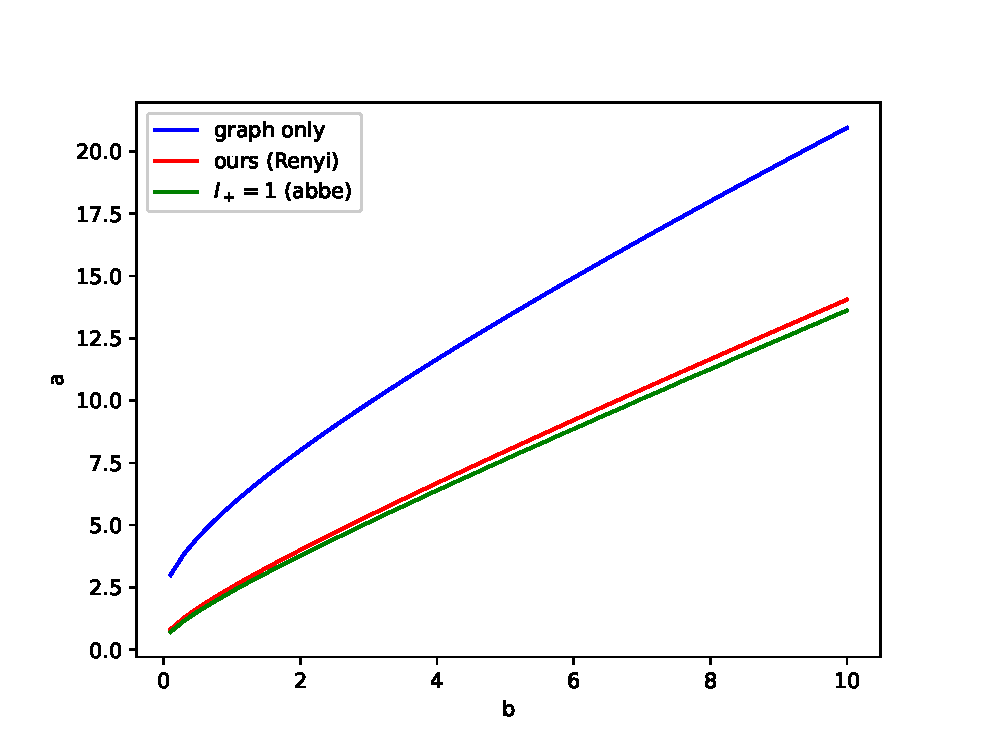
\includegraphics[width=0.6\textwidth]{comparison.eps}\caption{Theoretical comparison of different thresholds with $p_0 \sim \Bern(0.05), p_1\sim \Bern(0.5), \gamma=5$}
    \label{fig:my_label}
\end{figure}

The red line is our theoretical line
given by $a=(\sqrt{2 - \gamma D_{1/2}(p_0||p_1)} + \sqrt{b})^2$,
which is strictly over the green line. It tells that
exact recovery condition of Abbe is more stronger than us.
\subsection{Theoretical Equivalence}
Recall the definition of $g(\epsilon)$ as
	\begin{equation}\label{eq:gab}
	g(a,b,\epsilon) = a + b - \sqrt{\epsilon^2 + 4ab} + \epsilon \log \frac{\epsilon + \sqrt{\epsilon^2 + 4ab}}{2b}
	\end{equation}
	
We show that $I_+$ is equal to $\theta_1^*$.
\begin{align}
\theta^*_1 &= \min_{\widetilde{X}_1} \gamma D(p_{\widetilde{X}_1}|| p_0)+ \frac{1}{2} g(a,b, 2\epsilon)  \label{eq:theta}\\
\epsilon &= \gamma \frac{D(p_{\widetilde{X}_1} || P_1) - D(p_{\widetilde{X}_1} || P_0) }{\log a /b}\label{eq:equal}
\end{align}
We use Lagrange multiplier to solve \eqref{eq:theta}.
Let
$$
L(p_{\widetilde{X}_1},\epsilon, \lambda)
=\gamma D(p_{\widetilde{X}_1}|| p_0)+ \frac{1}{2} g(a,b, 2\epsilon) - \lambda(\epsilon \log\frac{a}{b}-\gamma
D(p_{\widetilde{X}_1} || P_1) + \gamma D(p_{\widetilde{X}_1} || P_0))
$$
It is equivalent to minimize
$(1-\lambda)D(p_{\widetilde{X}_1} || P_0) +
\lambda D(p_{\widetilde{X}_1} || P_1) $, from
which we get
\begin{equation}\label{eq:p12}
p_{\widetilde{X}_1}(x) = \frac{p_0^{1-\lambda}(x)p_1^{\lambda}(x)}{\sum_{x \in \mathcal{X}}p_0^{1-\lambda}(x) p_1^{\lambda} (x)}.
\end{equation}
From $\frac{\partial L(p_{\widetilde{X}_1},\epsilon, \lambda)}{\partial \epsilon}=0$ and taking \eqref{eq:p12}
into \eqref{eq:equal}, we get
\begin{align*}
    \lambda \log \frac{a}{b}
    & = \log \frac{\epsilon + \sqrt{\epsilon^2+ab}}{b} \\
    \epsilon \log \frac{a}{b}
    & = \gamma\frac{\sum_{x \in \mathcal{X}}p_0^{1-\lambda}(x) p_1^{\lambda} (x)\log \frac{p_0(x)}{p_1(x)}}{\sum_{x \in \mathcal{X}}p_0^{1-\lambda}(x) p_1^{\lambda} (x)}
\end{align*}
After cancelling $\epsilon$
from the above two equations, we can get a single equation
for $\lambda$:
\begin{equation}
    \frac{1}{2}\log\frac{a}{b}
    (a^{\lambda} b^{1-\lambda}
    -a^{1-\lambda} b^{\lambda})
    + \gamma \frac{\sum_{x \in \mathcal{X}}p_0^{1-\lambda}(x) p_1^{\lambda} (x)\log \frac{p_1(x)}{p_0(x)}}{\sum_{x \in \mathcal{X}}p_0^{1-\lambda}(x) p_1^{\lambda} (x)}=0
\end{equation}
which is the derivative of \eqref{eq:lambda}.
Then by simple computation we have
$I_+ = \theta_1^*$.
We can also show that $I_+=\theta_2^*$
where
\begin{align}
\theta^*_2 &= \min_{\widetilde{X}_1} \gamma D(p_{\widetilde{X}_2}|| p_1)+ \frac{1}{2} g(a,b, 2\epsilon)  \label{eq:theta2}\\
\epsilon &= \gamma \frac{D(p_{\widetilde{X}_2} || P_0) - D(p_{\widetilde{X}_2} || P_1) }{\log a /b}\label{eq:equal2}
\end{align}
We use Lagrange multiplier to solve \eqref{eq:theta2}.
Let
$$
L(p_{\widetilde{X}_2},\epsilon, \lambda)
=\gamma D(p_{\widetilde{X}_2}|| p_1)+ \frac{1}{2} g(a,b, 2\epsilon) - (1-\lambda)(\epsilon \log\frac{a}{b}-\gamma
D(p_{\widetilde{X}_2} || P_0) + \gamma D(p_{\widetilde{X}_2} || P_1))
$$
It is equivalent to minimize
$(1-\lambda)D(p_{\widetilde{X}_2} || P_0) +
\lambda D(p_{\widetilde{X}_2} || P_1) $, from
which we get
\begin{equation}\label{eq:p122}
p_{\widetilde{X}_2}(x) = \frac{p_0^{1-\lambda}(x)p_1^{\lambda}(x)}{\sum_{x \in \mathcal{X}}p_0^{1-\lambda}(x) p_1^{\lambda} (x)}.
\end{equation}
From $\frac{\partial L(p_{\widetilde{X}_2},\epsilon, \lambda)}{\partial \epsilon}=0$ and taking \eqref{eq:p122}
into \eqref{eq:equal2}, we get
\begin{align*}
    (1-\lambda) \log \frac{a}{b}
    & = \log \frac{\epsilon + \sqrt{\epsilon^2+ab}}{b} \\
    \epsilon \log \frac{a}{b}
    & = \gamma\frac{\sum_{x \in \mathcal{X}}p_0^{1-\lambda}(x) p_1^{\lambda} (x)\log \frac{p_1(x)}{p_0(x)}}{\sum_{x \in \mathcal{X}}p_0^{1-\lambda}(x) p_1^{\lambda} (x)}
\end{align*}
After cancelling $\epsilon$
from the above two equations, we can get a single equation
for $\lambda$:
\begin{equation}
    \frac{1}{2}\log\frac{a}{b}
    (a^{\lambda} b^{1-\lambda}
    -a^{1-\lambda} b^{\lambda})
    + \gamma \frac{\sum_{x \in \mathcal{X}}p_0^{1-\lambda}(x) p_1^{\lambda} (x)\log \frac{p_1(x)}{p_0(x)}}{\sum_{x \in \mathcal{X}}p_0^{1-\lambda}(x) p_1^{\lambda} (x)}=0
\end{equation}
which is the derivative of \eqref{eq:lambda}.
Then by simple computation we have
$I_+ = \theta_2^*$.

Let $\theta^*_3 = \frac{1}{2}[\gamma D_{1/2}(p_0||p_1) + (\sqrt{a} - \sqrt{b})^2]$.
We can verify that $\theta_1^*=\theta_2^*>\theta^*_3$.
A prove of this conclusion is considering
linear approximation of $g(a,b,2\epsilon)$
in \eqref{eq:theta2}.
\begin{equation}\label{eq:g_linear}
		g(a,b,\epsilon) \geq  (\sqrt{a} - \sqrt{b})^2 + \frac{\epsilon}{2}\log \frac{a}{b}. 
	\end{equation}
	Then, by Lemma \ref{lem:p0p12},
	\begin{align*}
		\theta^*_1 \geq \frac{1}{2}(\sqrt{a}-\sqrt{b})^2+\gamma \frac{D(P_{\widetilde{X}_1} || P_1) + D(P_{\widetilde{X}_1} || P_0)}{2} \\
		\geq \frac{1}{2}((\sqrt{a}-\sqrt{b})^2+\gamma D_{1/2}(P_0||P_1))=\theta^*_3,
	\end{align*}
	where the equality holds when $P_{\widetilde{X}_1}$ is given by \eqref{eq:p012}. 
	\begin{lemma}\label{lem:p0p12}
		Let $P_1, P_2$ be two different
        probability distribution functions defined over $\mathcal{X}$.
        The minimizer
		of $D(P_{\lambda}||P_1) + 
        D(P_{\lambda}||P_2)$ 
        over $0<\lambda < 1$
        (The definition of $P_{\lambda}$
        can be seen from \eqref{eq:P_lambda})
        is achieved when $\lambda=\frac{1}{2}$,
        then the PMF of $P_{\lambda}$ has the following form:
		\begin{equation}\label{eq:p012}
			P(X=x)=\frac{\sqrt{P_1(x)
            P_2(x)}}
            { \sum_{y\in \mathcal{X}} 
            \sqrt{P_1(y)
                P_2(y)}
            }
		\end{equation}
		and the minimal value is
		$-2\log \sum_{x\in \mathcal{X}} 
        \sqrt{P_1(x) P_2(x)}$.
	\end{lemma}
\begin{proof}
    Let $H(\lambda)=D(P_{\lambda}||P_1) + 
    D(P_{\lambda}||P_2), C(\lambda)=\sum_{y \in \mathcal{X}}
    P_1^{1-\lambda}(y)
    P_2^{\lambda} (y)$.
    Then
    \begin{equation}
        H(\lambda)
        = \sum_{x\in \mathcal{X}}
        (1-2\lambda)\frac{P^{1-\lambda}_1(x)P^{\lambda}_2(x)}
        {C(\lambda)}\frac{P_1(x)}
        {P_2(x)} - 2 \log C(\lambda)
    \end{equation}
    The first derivative of $H(\lambda)$ is
    \begin{equation}
        H'(\lambda) = \frac{1-2\lambda}{C^2}
        \left[
            \left(\sum_{x\in \mathcal{X}}
            P_1^{1-\lambda}(x)
            P_2^{\lambda}(x) \log\frac{P_2(x)}{P_1(x)}
            \right)^2
            - C \sum_{x\in \mathcal{X}}P_1^{1-\lambda}(x)
            P_2^{\lambda}(x) \log\frac{P^2_2(x)}{P^2_1(x)}
        \right]
    \end{equation}
    By Cauchy's inequality and $P_1\neq P_2$,
    the term inside the
    square bracket is negative.
    Therefore, $H'(\lambda)$ is monotonic increasing within
    the interval $(0,1)$. Since $H'(\lambda)=0$,
    $H(\lambda)$ achieves its minimal value at $\lambda=\frac{1}{2}$.
    Finally, we can verify that 
    $H(\frac{1}{2})=-2\log \sum_{x\in \mathcal{X}} 
    \sqrt{P_1(x) P_2(x)}$.
\end{proof}
\begin{thebibliography}{9}
\bibitem{kl} https://stats.stackexchange.com/questions/145789/kl-divergence-between-two-univariate-poisson-distributions
\bibitem{abbe} Asadi, Amir R., Emmanuel Abbe, and Sergio Verdú. "Compressing data on graphs with clusters." 2017 IEEE International Symposium on Information Theory (ISIT). IEEE, 2017.
\end{thebibliography}
\end{document}

